\section{Chairs}
\begin{figure}[h]
\centering
\subfloat[]{
	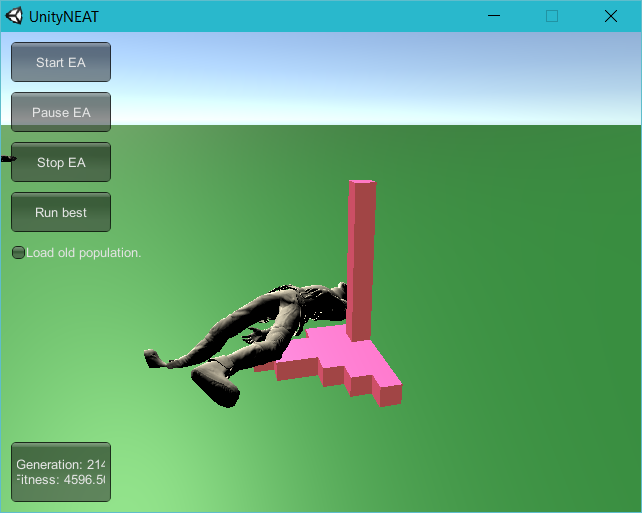
\includegraphics[width=.9\columnwidth, trim={80 0 80 60}, clip]{chair_leg}
}
\hfil
\subfloat[]{
	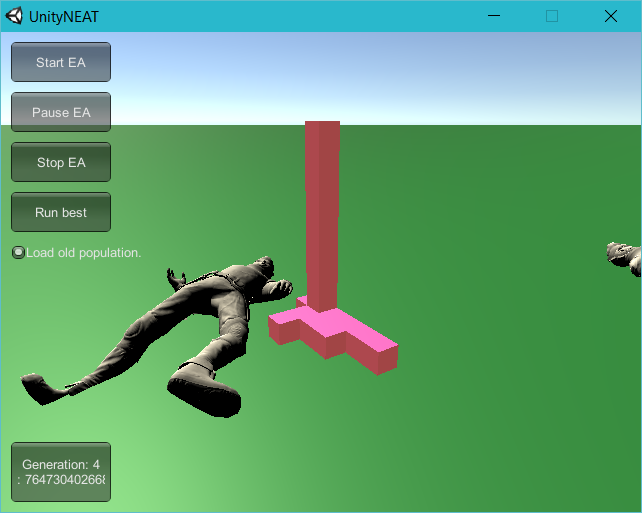
\includegraphics[width=.9\columnwidth, trim={80 0 80 30}, clip]{chair_leg2}
}
\caption{Example showing how individuals can evolve to chair legs.}
\label{fig:chair:legs}
\end{figure}

\begin{figure}[h]
\centering
\subfloat[]{
	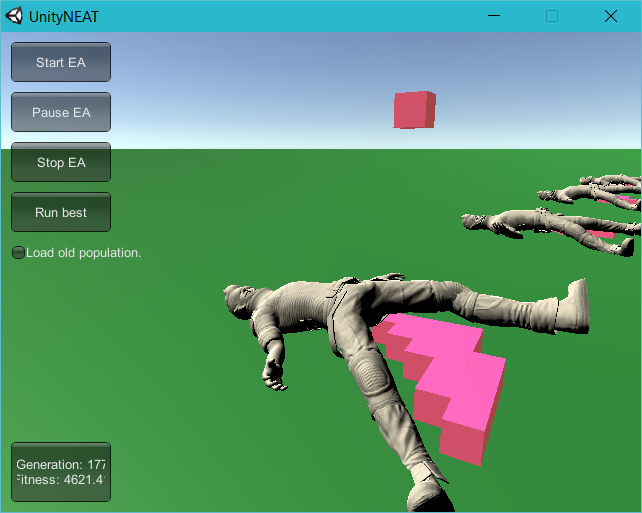
\includegraphics[width=.9\columnwidth, trim={80 0 0 30}, clip]{floating_voxel}
}
\caption{Example showing a floating voxel, this should in theory not happen.}
\label{fig:chair:floatvox}
\end{figure}

\begin{figure}[h]
\centering
\subfloat[]{
	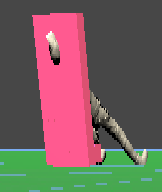
\includegraphics[height=70pt]{metro_stand}
}
\caption{Example showing a floating voxel, this should in theory not happen.}
\label{fig:chair:floatvox}
\end{figure}
